\section{Cơ sở lý thuyết và hệ thống liên quan}
\label{sec:background}
\begingroup
\setlength{\parskip}{3.5pt}
\setstretch{1.15}

\subsection{Nội dung văn hóa và truy nguyên nguồn}
Trong CultureMap VN, địa phương và chủ đề là các điểm truy cập nội dung.
Một bài giới thiệu cần gắn đối tượng văn hóa với câu chuyện và bối cảnh;
nguồn tham khảo cung cấp căn cứ để kiểm tra từng phần thông tin.
Hồ sơ Nhã nhạc của UNESCO minh họa cách nhận diện tài liệu thông qua tên,
mã hồ sơ và thông tin ghi danh \cite{unesco-nhanhac}.

Việc truy nguyên cần phân biệt tài liệu gốc, nội dung biên soạn và phản
hồi do AI tạo. Thông tin nguồn gồm tên tài liệu, tác giả hoặc đơn vị phát
hành, thời điểm, địa chỉ truy cập và ngày truy cập. Mối liên hệ giữa nguồn
với dữ kiện có ý nghĩa trực tiếp đối với đối chiếu nội dung và đánh giá AI.

\subsection{Hỏi đáp dựa trên dữ liệu và các hướng tiếp cận AI}
\subsubsection{Sinh câu trả lời kết hợp truy xuất}
Retrieval-Augmented Generation (RAG) kết hợp truy xuất thông tin bên ngoài
với mô hình sinh ngôn ngữ. Công trình của Lewis và cộng sự mô tả sự kết
hợp giữa tri thức trong tham số mô hình và bộ nhớ ngoài được truy xuất
\cite{lewis-rag}. Trong bài toán của đề tài, hướng này được xem xét để đưa
nội dung phù hợp vào ngữ cảnh trả lời, gắn kết quả với bằng chứng.

Tìm được tài liệu liên quan chưa bảo đảm câu trả lời đúng. Phần truy xuất
cần chọn được bằng chứng phù hợp; phần sinh cần sử dụng đúng bằng chứng,
thể hiện căn cứ và xử lý câu hỏi ngoài phạm vi. Đây là hai khía cạnh
được xem xét khi thiết kế đánh giá.

\subsubsection{RAG và fine-tuning trong phạm vi đồ án}
RAG đưa tư liệu được truy xuất vào ngữ cảnh trả lời; bản thân bước này
không thay đổi trọng số mô hình. Fine-tuning là tiếp tục huấn luyện một
mô hình có sẵn bằng các ví dụ phù hợp với một nhiệm vụ. Hai kỹ thuật tác
động đến hệ thống theo những cách khác nhau và có thể được xem xét kết hợp.

Nhóm dự định thực hiện cả RAG và fine-tuning ở quy mô nhỏ. RAG phục vụ hỏi
đáp có căn cứ từ nội dung bài; nhiệm vụ cụ thể của fine-tuning, cách chuẩn
bị ví dụ và vị trí sử dụng mô hình sau tinh chỉnh sẽ được thống nhất tại
Chương~\ref{sec:ai}. Chưa mặc định fine-tuning cải thiện kết quả hoặc thay
thế việc dẫn nguồn; nhận định cần dựa trên đánh giá thực tế.

\subsubsection{Đánh giá chất lượng}
Các hướng đánh giá gồm mức độ tìm được bằng chứng cần thiết, tính đúng
của câu trả lời, mức được bằng chứng hỗ trợ và sự phù hợp của dẫn nguồn.
Bộ kiểm tra có thể phân biệt trường hợp có đủ thông tin, thiếu thông tin
và ngoài phạm vi; độ trễ, chi phí và lỗi dịch vụ là các yếu tố cần cân nhắc.
Các khái niệm này làm cơ sở thảo luận giải pháp ở
Chương~\ref{sec:ai}. Với fine-tuning, cần tách dữ liệu huấn luyện và
đánh giá, so sánh mô hình trước/sau trên cùng nhiệm vụ. Phạm vi giới hạn ở
thử nghiệm nhỏ, không huấn luyện mô hình từ đầu.

\subsection{Khảo sát các hệ thống liên quan}
Đối chiếu sử dụng giao diện công khai của Vietnam Tourism, UNESCO ICH,
Google Arts \& Culture và Bảo tàng Mỹ thuật Việt Nam. Các tiêu chí gồm
cách truy cập nội dung, tổ chức thông tin, trình bày tư liệu và khả năng
truy nguyên nguồn. Mỗi hệ thống được minh họa bằng một ảnh giao diện;
nhận xét giới hạn ở những trang đã khảo sát.
\par\endgroup

\clearpage
\subsubsection{Vietnam Tourism: khám phá theo điểm đến và chủ đề}
Chuyên mục Culture \& Heritage sử dụng thanh tìm kiếm, nhóm trải nghiệm
và các thẻ bài viết để dẫn người đọc tới nội dung \cite{vietnam-culture}.
Hình~\ref{fig:reference-vietnam-tourism} minh họa cách tổ chức giao diện này.

\begin{figure}[H]
\centering
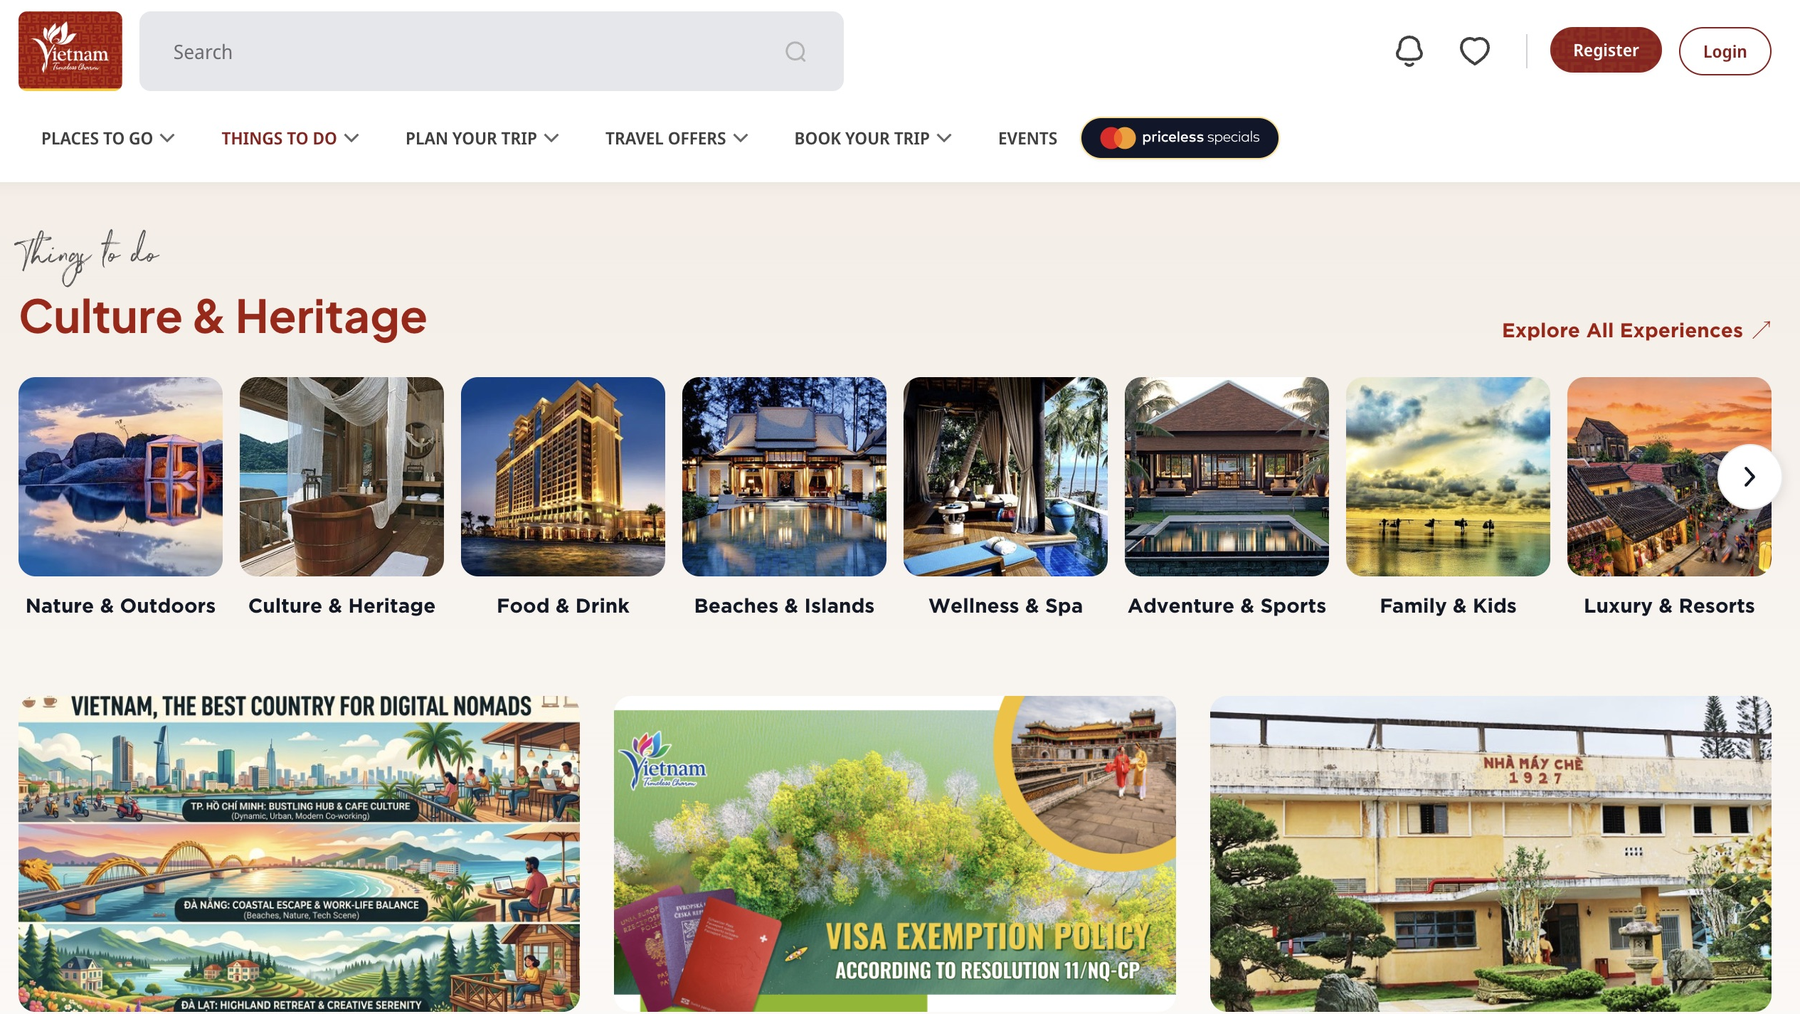
\includegraphics[width=0.94\linewidth,height=60mm,keepaspectratio]{assets/references/vietnam-tourism-interface.png}
\caption{Giao diện chuyên mục Culture \& Heritage của Vietnam Tourism}
\label{fig:reference-vietnam-tourism}
\par\smallskip{\footnotesize Nguồn: Vietnam Tourism \cite{vietnam-culture}; ảnh chụp ngày 01/11/2026.}
\end{figure}

Đối với CultureMap VN, điểm tham khảo là lối vào theo chủ đề và cách
trình bày kết quả bằng các thẻ nội dung. Thông tin địa phương, giới thiệu
ngắn và nguồn tham khảo cần giúp người đọc quyết định mở bài và kiểm tra.

\subsubsection{UNESCO ICH: hồ sơ có nhận diện và bối cảnh}
Hồ sơ Nhã nhạc trên UNESCO ICH trình bày tên di sản, mã hồ sơ và thông
tin ghi danh \cite{unesco-nhanhac}. Hình~\ref{fig:reference-unesco} thể
hiện sự tách biệt giữa nhận diện hồ sơ và thông tin mô tả.

\begin{figure}[H]
\centering
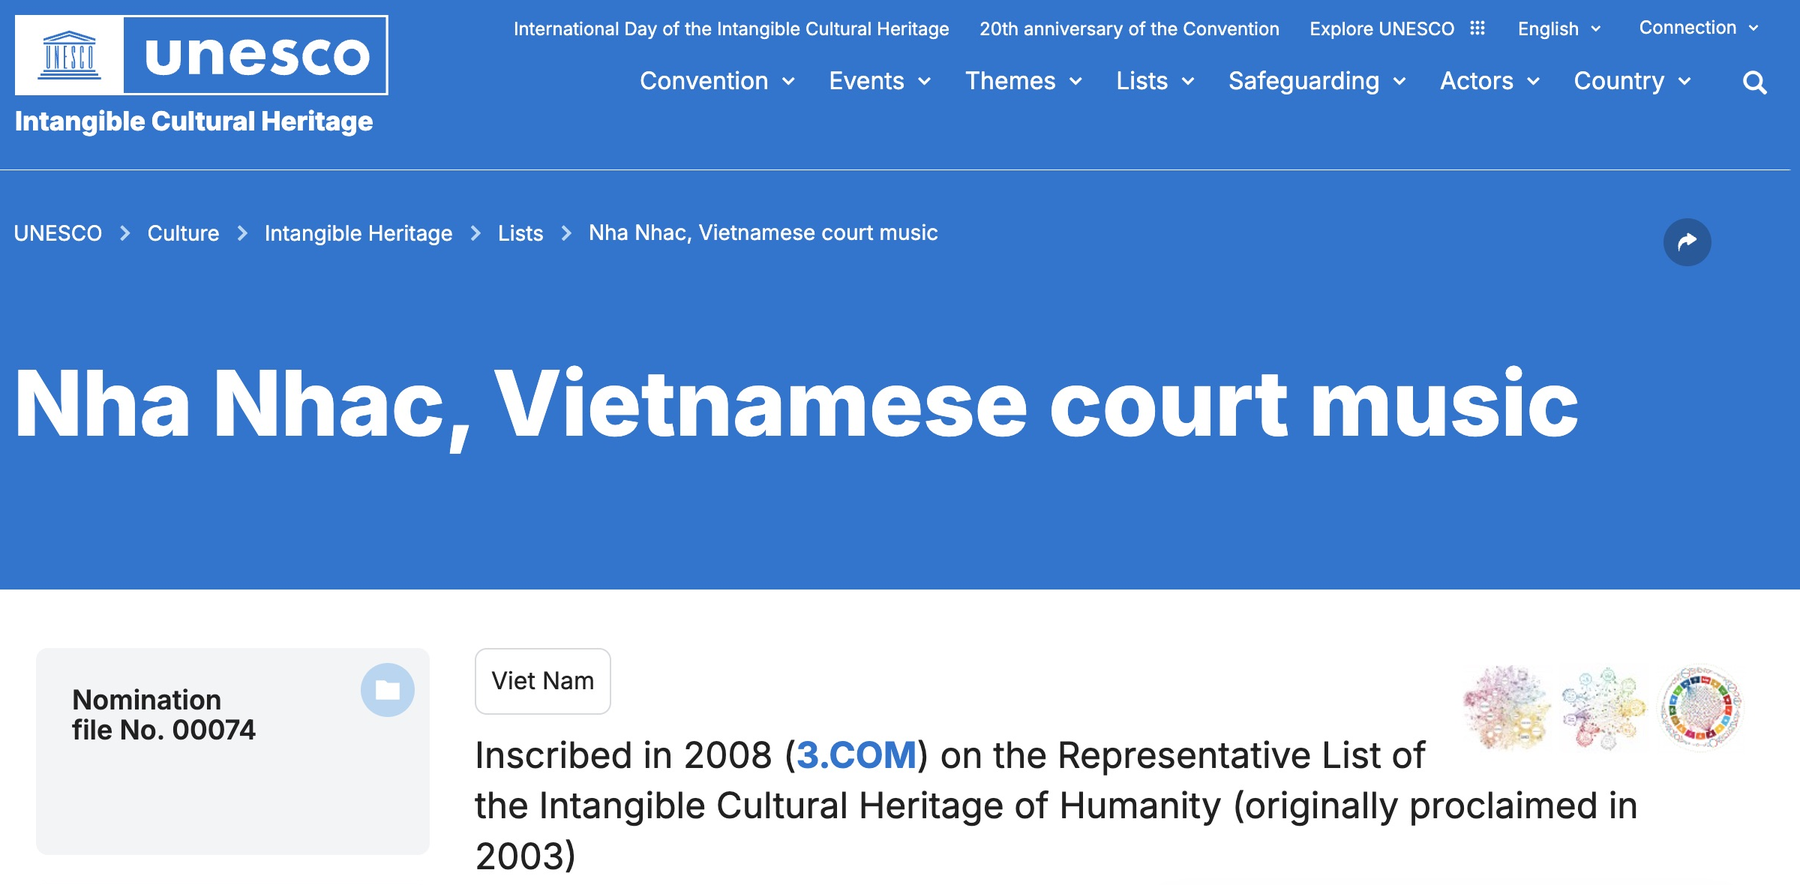
\includegraphics[width=0.94\linewidth,height=60mm,keepaspectratio]{assets/references/unesco-ich-interface.png}
\caption{Giao diện hồ sơ Nhã nhạc trên UNESCO Intangible Cultural Heritage}
\label{fig:reference-unesco}
\par\smallskip{\footnotesize Nguồn: UNESCO ICH \cite{unesco-nhanhac}; ảnh chụp ngày 01/11/2026.}
\end{figure}

CultureMap VN có thể vận dụng cách nhận diện tài liệu để trình bày nguồn
và bối cảnh dữ kiện. Bài biên soạn cần liên kết với nguồn hỗ trợ; kết quả
đối chiếu được ghi theo tài liệu sử dụng và có thể kiểm tra lại.

\clearpage
\subsubsection{Google Arts \& Culture: khám phá qua câu chuyện và tư liệu}
Dự án Wonders of Vietnam giới thiệu các chủ đề văn hóa qua hình ảnh,
câu chuyện và những lối khám phá liên quan \cite{google-wonders}.
Hình~\ref{fig:reference-google-arts} minh họa trang giới thiệu dự án.

\begin{figure}[H]
\centering
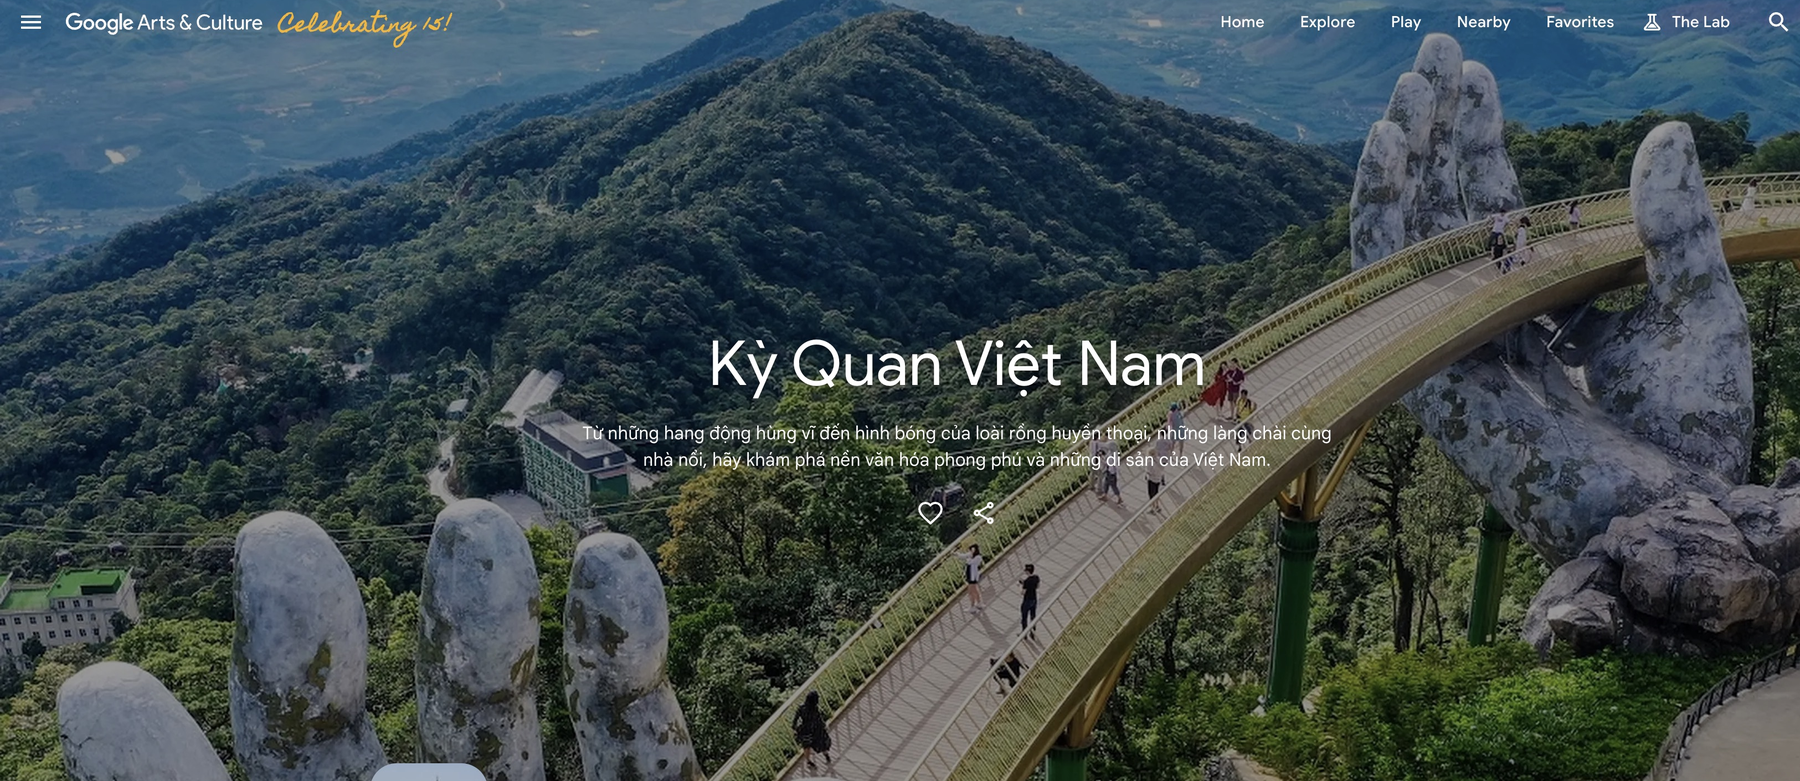
\includegraphics[width=0.94\linewidth,height=60mm,keepaspectratio]{assets/references/google-arts-culture-interface.png}
\caption{Giao diện dự án Kỳ quan Việt Nam trên Google Arts \& Culture}
\label{fig:reference-google-arts}
\par\smallskip{\footnotesize Nguồn: Google Arts \& Culture \cite{google-wonders}; ảnh chụp ngày 01/11/2026.}
\end{figure}

Điểm tham khảo là cách kết nối đối tượng với câu chuyện và tư liệu. Ví dụ,
bài về gốm Thanh Hà gắn sản phẩm với nguyên liệu và công đoạn
\cite{google-thanhha}. CultureMap VN vận dụng cách tiếp cận này để tổ chức
bài giới thiệu và hỗ trợ hỏi thêm theo ngữ cảnh.

\subsubsection{Bảo tàng Mỹ thuật Việt Nam: tổ chức nội dung theo sưu tập}
Website Bảo tàng Mỹ thuật Việt Nam có các lối truy cập Trưng bày, Sưu tập
và 3D Tour \cite{vietnam-fine-arts}. Hình~\ref{fig:reference-fine-arts}
minh họa giao diện trang chủ với các nhóm nội dung và triển lãm trực tuyến.

\begin{figure}[H]
\centering
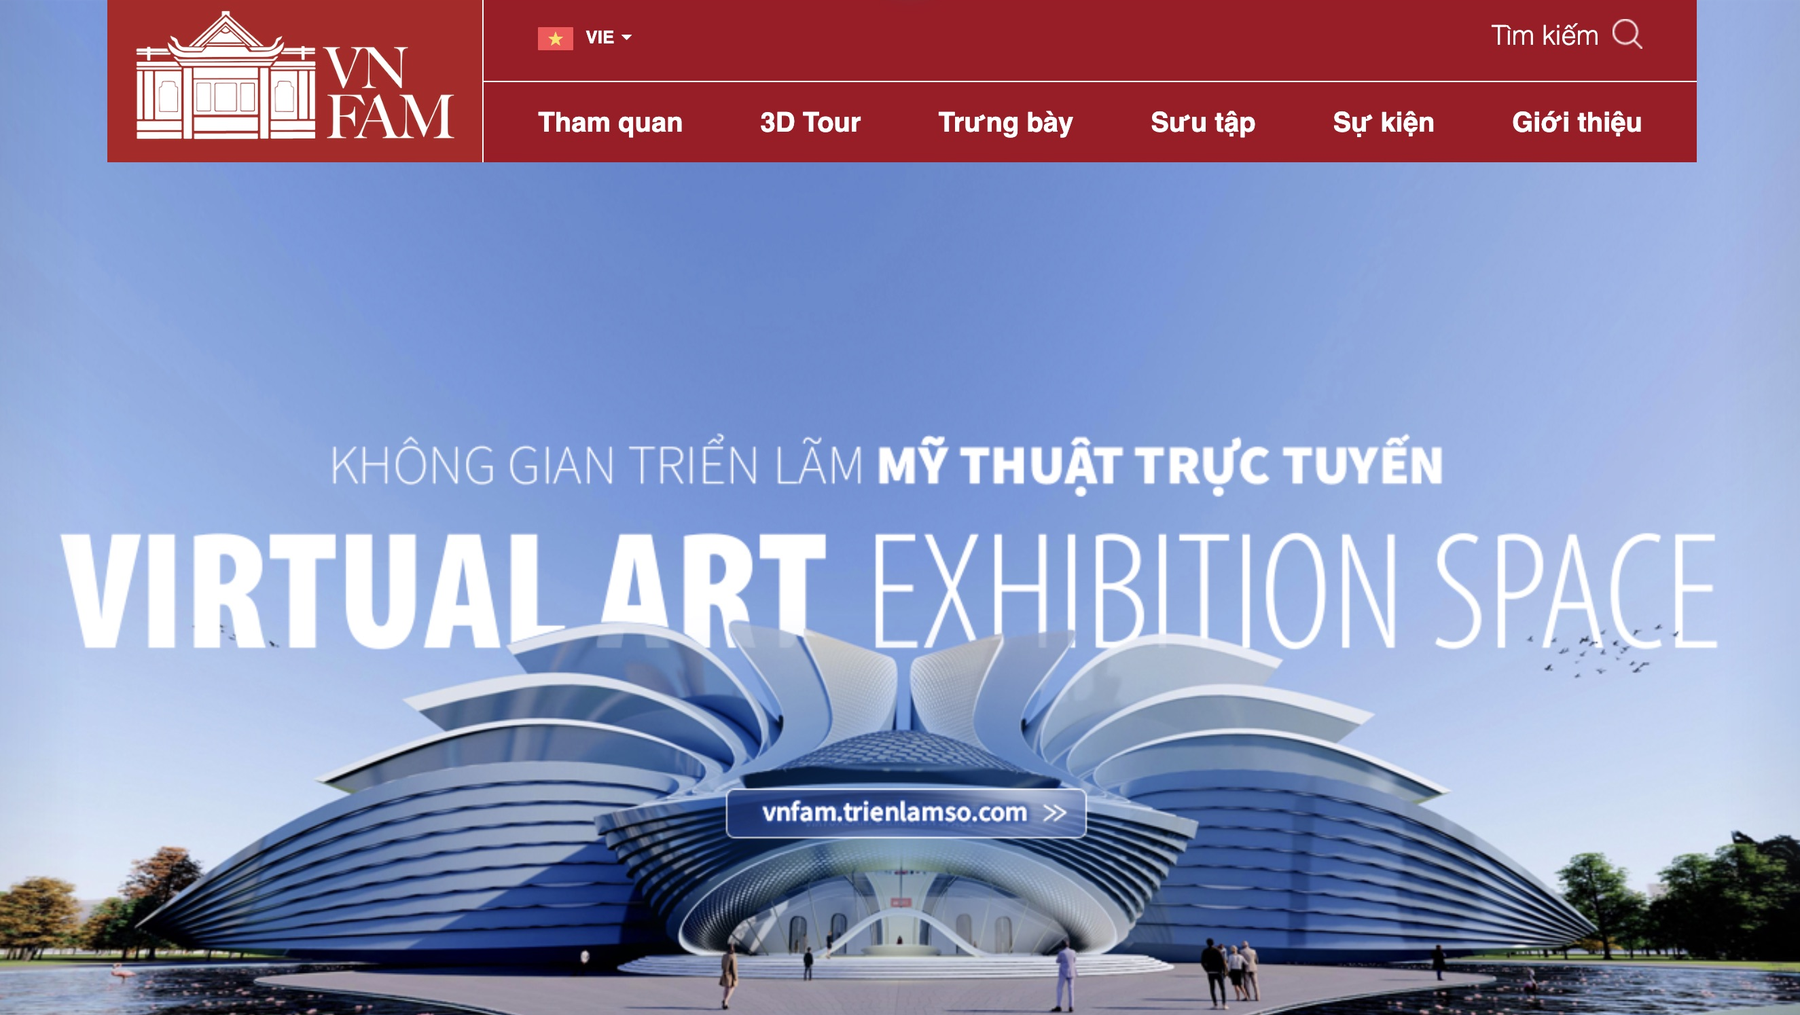
\includegraphics[width=0.94\linewidth,height=60mm,keepaspectratio]{assets/references/vietnam-fine-arts-museum-interface.png}
\caption{Giao diện website Bảo tàng Mỹ thuật Việt Nam}
\label{fig:reference-fine-arts}
\par\smallskip{\footnotesize Nguồn: Bảo tàng Mỹ thuật Việt Nam \cite{vietnam-fine-arts}; ảnh chụp ngày 01/11/2026.}
\end{figure}

CultureMap VN tham khảo cách phân nhóm đối tượng và dẫn người đọc từ
một nhóm nội dung tới đối tượng cụ thể. Việc kết hợp tìm kiếm, phân loại
và tư liệu có xuất xứ giúp hình thành trải nghiệm khám phá có trình tự.
